\newpage
\section{Разностная схема}
\subsection{Описание схемы}

Для поиска численного решения задачи $(1)$ можно использовать разностную схему, в которой при апроксимации конвективных членов используются центральные разности, а приближенные значения плотности $H$ и скорости $V$ на каждом временном слое ищутся в узлах сетки $\Omega_h$ как решения двух СЛАУ, порядок решения которых произволен:

$$H_t + 0.5\sum_{k=1}^2(V_k\hat{H}_{\mathring{x}_k} + (V_k\hat{H})_{\mathring{x}_k} + H(V_k)_{\mathring{x}_k}) = 0, w \in \Omega_h \eqno(2.1)$$

$$H_t + 0.5((V_k\hat{H})_{x_k} + H(V_k)_{x_k}) - 0.5h_k((HV_k)_{x_k\bar{x}_k}^{+1_k} - 0.5(HV_k)_{x_k\bar{x}_k}^{+2_k} + $$
$$+ H((V_k)_{x_k\bar{x}_k}^{^+1_k} - 0.5(V_k)_{x_k\bar{x}_k}^{+2_k})) = 0, x \in \gamma_k^-  \eqno(2.2)$$

$$H_t + 0.5((V_k\hat{H})_{\bar{x}_k} + H(V_k)_{\bar{x}_k}) - 0.5h_k((HV_k)_{x_k\bar{x}_k}^{-1_k} - 0.5(HV_k)_{x_k\bar{x}_k}^{-2_k} + $$
$$ + H((V_k)_{x_k\bar{x}_k}^{^-1_k} - 0.5(V_k)_{x_k\bar{x}_k}^{-2_k})) = 0, x \in \gamma_k^-  \eqno(2.3)$$

$$(V_k)_t + \frac{1}{3}(V_k(\hat{V}_k)_{\mathring{x}_k} + (V_k\hat{V}_k)_{\mathring{x}_k}) + $$
$$\frac{1}{2}\sum_{m=1, m\neq k}^2 \left(V_m(\hat{V}_k)_{\mathring{x}_m} + (V_m\hat{V}_k)_{\mathring{x}_m} - V_k(V_m)_{\mathring{x}_m} \right) + \frac{p(H)_{\mathring{x}_k}}{H} = $$
$$ = \tilde{\mu}\left(\frac{4}{3}(\hat{V}_k)_{x_k\bar{x}_k} + \sum_{m=1, m\neq k}^{2} (\hat{V}_k)_{x_m\bar{x}_m}\right) - (\tilde{\mu} - \frac{\mu}{H})\left(\frac{4}{3}(V_k)_{x_k\bar{x}_k} + \sum_{m=1, m\neq k}^{2} (V_k)_{x_m\bar{x}_m}\right) + $$
$$ + \frac{\mu}{3H}\sum_{m=1, m\neq k}^{2}(V_m)_{\mathring{x}_k\mathring{x}_m} + f_k, x\in \Omega_h  \eqno(2.4)$$

$$\hat{V}_k = 0, x \in \gamma_{h}^-, k=1,2  \eqno(2.5)$$

Где:
$$\tilde{\mu} = \max_m \frac{\mu}{H}$$

\subsection{Координатная запись}
Распишем схему приведенных выше обозначениях, и выделим коэффиценты при $H\,$ и $V$ на $n + 1$ временном слое:
\subsubsection{1 уравнение (2.1)}
$$H_t + 0.5\sum_{k=1}^2(V_k\hat{H}_{\mathring{x}_k} + (V_k\hat{H})_{\mathring{x}_k} + H(V_k)_{\mathring{x}_k}) = 0$$\\

$
2\frac{H^{n+1}_{m_1, m_2} - H^n_{m_1, m_2}}{\tau} + V_{1 \, m_1, m_2}^n \frac{H_{m_1 + 1, m_2}^{n+1} - H_{m_1 - 1, m_2}^{n+1}}{2h_1} + \frac{V_{1 \, m_1+1, m_2}^nH_{m_1+1, m_2}^{n+1} - V_{1 \, m_1-1, m_2}^nH_{m_1-1, m_2}^{n+1}}{2h_1} + \\
+ H_{m_1, m_2}^n\left(\frac{V_{1 \, m_1 + 1, m_2}^n - V_{1 \, m_1 - 1, m_2}^n}{2h_1}\right) + \\
+ V_{2 \, m_1, m_2}^n \frac{H_{m_1, m_2 + 1}^{n+1} - H_{m_1, m_2 - 1}^{n+1}}{2h_2} + \frac{V_{2 \, m_1, m_2+1}^nH_{m_1, m_2+1}^{n+1} - V_{2 \, m_1, m_2-1}^nH_{m_1, m_2 - 1}^{n+1}}{2h_2} + \\
+ H_{m_1, m_2}^n\left(\frac{V_{2 \, m_1, m_2 + 1}^n - V_{2 \, m_1, m_2 - 1}^n}{2h_2}\right) = 0
$\\

$
H_{m_1 - 1, m_2}^{n+1} (-\frac{V_{1 \, m_1, m_2}^n + V_{1 \, m_1 - 1, m_2}^n}{2h_1}) + H_{m_1, m_2}^{n+1}(\frac{2}{\tau}) + H_{m_1 + 1, m_2}^{n+1}(\frac{V_{1 \, m_1, m_2}^n + V_{1 \, m_1 + 1, m_2}^n}{2h_1}) + \\
+ H_{m_1, m_2 - 1}^{n+1} (-\frac{V_{2 \, m_1, m_2}^n + V_{2 \, m_1, m_2 - 1}^n}{2h_2}) + H_{m_1, m_2}^{n+1}(0) + H_{m_1, m_2 + 1}^{n+1}(\frac{V_{2 \, m_1, m_2}^n + V_{1 \, m_1, m_2 + 1}^n}{2h_2}) = \\
= -\frac{2H_{m_1, m_2}^n}{\tau} - H_{m_1, m_2}^n \left(\frac{V_{1 \, m_1 + 1, m_2}^n - V_{1 \, m_1 - 1, m_2}^n}{2h_1} + \frac{V_{2 \, m_1, m_2 + 1}^n - V_{2 \, m_1, m_2 - 1}^n}{2h_2}\right)
$\\

\newpage
\subsubsection{2 уравнение (2.2)}
$$H_t + 0.5((V_k\hat{H})_{x_k} + H(V_k)_{x_k}) - 0.5h_k((HV_k)_{x_k\bar{x}_k}^{+1_k} - 0.5(HV_k)_{x_k\bar{x}_k}^{+2_k} + $$
$$+ H((V_k)_{x_k\bar{x}_k}^{^+1_k} - 0.5(V_k)_{x_k\bar{x}_k}^{+2_k})) = 0$$\\

Распишем случай для $k = 1$:
$$H_t + 0.5((V_1\hat{H})_{x_1} + H(V_1)_{x_1}) - 0.5h_1((HV_1)_{x_1\bar{x}_1}^{+1_1} - 0.5(HV_1)_{x_1\bar{x}_1}^{+2_1} + $$
$$+ H((V_1)_{x_1\bar{x}_1}^{^+1_1} - 0.5(V_1)_{x_1\bar{x}_1}^{+2_1})) = 0$$\\

$
\frac{H^{n+1}_{m_1, m_2} - H^n_{m_1, m_2}}{\tau} + 0.5(\frac{V_{1 \, m_1 + 1, m_2}^nH_{m_1 + 1, m_2}^{n+1} - V_{1 \, m_1, m_2}^nH_{m_1, m_2}^{n+1}}{h_1} + H_{m_1, m_2}^n\frac{V_{1 \, m_1 + 1, m_2}^n - V_{1 \, m_1, m_2}^n}{h_1}) - \\
- 0.5h_1((\frac{H_{m_1, m_2}^nV_{1 \, m_1, m_2}^n - 2H_{m_1 + 1, m_2}^nV_{1 \, m_1 + 1, m_2}^n + H_{m_1+2, m_2}^nV_{1 \, m_1+2, m_2}^n}{h_1^2}) - \\
- 0.5\frac{H_{m_1+1, m_2}^nV_{1 \, m_1+1, m_2}^n - 2H_{m_1 + 2, m_2}^nV_{1 \, m_1 + 2, m_2}^n + H_{m_1+3, m_2}^nV_{1 \, m_1+3, m_2}^n}{h_1^2} + \\
+ H_{m_1, m_2}^n(\frac{V_{1 \, m_1, m_2}^n - 2V_{1 \, m_1 + 1, m_2}^n + V_{1 \, m_1+2, m_2}^n}{h_1^2} - 0.5\frac{V_{1 \, m_1 + 1, m_2}^n - 2V_{1 \, m_1 + 2, m_2}^n + V_{1 \, m_1+3, m_2}^n}{h_1^2})) = 0
$\\

$
H_{m_1 - 1, m_2}^{n+1} (0) + H_{m_1, m_2}^{n+1}(\frac{1}{\tau} - 0.5\frac{V_{1 \, m_1, m_2}^n}{h_1}) + H_{m_1 + 1, m_2}^{n+1}(0.5\frac{V_{1 \, m_1 + 1, m_2}^n}{h_1}) + \\
+ H_{m_1, m_2 - 1}^{n+1} (0) + H_{m_1, m_2}^{n+1}(0) + H_{m_1, m_2 + 1}^{n+1}(0) =\\
= -0.5H_{m_1, m_2}^n\frac{V_{1 \, m_1+1, m_2}^n - V_{1 \, m_1, m_2}^n}{h_1} + \frac{H_{m_1, m_2}^n}{\tau} +\\
+ 0.5h_1((\frac{H_{m_1, m_2}^nV_{1 \, m_1, m_2}^n - 2H_{m_1 + 1, m_2}^nV_{1 \, m_1 + 1, m_2}^n + H_{m_1+2, m_2}^nV_{1 \, m_1+2, m_2}^n}{h_1^2}) - \\
- 0.5\frac{H_{m_1+1, m_2}^nV_{1 \, m_1+1, m_2}^n - 2H_{m_1 + 2, m_2}^nV_{1 \, m_1 + 2, m_2}^n + H_{m_1+3, m_2}^nV_{1 \, m_1+3, m_2}^n}{h_1^2} + \\
+ H_{m_1, m_2}^n(\frac{V_{1 \, m_1, m_2}^n - 2V_{1 \, m_1 + 1, m_2}^n + V_{1 \, m_1+2, m_2}^n}{h_1^2} - 0.5\frac{V_{1 \, m_1 + 1, m_2}^n - 2V_{1 \, m_1 + 2, m_2}^n + V_{1 \, m_1+3, m_2}^n}{h_1^2}))
$\\

\newpage
Распишем случай для $k = 2$:
$$H_t + 0.5((V_2\hat{H})_{x_2} + H(V_2)_{x_2}) - 0.5h_2((HV_2)_{x_2\bar{x}_2}^{+1_2} - 0.5(HV_2)_{x_2\bar{x}_2}^{+2_2} + $$
$$+ H((V_2)_{x_2\bar{x}_2}^{^+1_2} - 0.5(V_2)_{x_2\bar{x}_2}^{+2_2})) = 0$$\\

$
\frac{H^{n+1}_{m_1, m_2} - H^n_{m_1, m_2}}{\tau} + 0.5(\frac{V_{2 \, m_1, m_2+1}^nH_{m_1, m_2+1}^{n+1} - V_{2 \, m_1, m_2}^nH_{m_1, m_2}^{n+1}}{h_2} + H_{m_1, m_2}^n\frac{V_{2 \, m_1, m_2+1}^n - V_{2 \, m_1, m_2}^n}{h_2}) - \\
- 0.5h_2((\frac{H_{m_1, m_2}^nV_{2 \, m_1, m_2}^n - 2H_{m_1, m_2 + 1}^nV_{2 \, m_1, m_2 + 1}^n + H_{m_1, m_2+2}^nV_{2 \, m_1, m_2+2}^n}{h_2^2}) - \\
- 0.5\frac{H_{m_1, m_2+1}^nV_{2 \, m_1, m_2+1}^n - 2H_{m_1, m_2 + 2}^nV_{2 \, m_1, m_2 + 2}^n + H_{m_1, m_2+3}^nV_{2 \, m_1, m_2+3}^n}{h_2^2} + \\
+ H_{m_1, m_2}^n(\frac{V_{2 \, m_1, m_2}^n - 2V_{2 \, m_1, m_2+1}^n + V_{2 \, m_1, m_2+2}^n}{h_2^2} - 0.5\frac{V_{2 \, m_1, m_2+1}^n - 2V_{2 \, m_1, m_2+2}^n + V_{2 \, m_1, m_2+3}^n}{h_2^2})) = 0
$\\

$
H_{m_1 - 1, m_2}^{n+1} (0) + H_{m_1, m_2}^{n+1}(0) + H_{m_1 + 1, m_2}^{n+1}(0) + \\
+ H_{m_1, m_2 - 1}^{n+1} (0) + H_{m_1, m_2}^{n+1}(\frac{1}{\tau} - 0.5\frac{V_{2 \, m_1, m_2}^n}{h_2}) + H_{m_1, m_2 + 1}^{n+1}(0.5\frac{V_{2 \, m_1, m_2+1}^n}{h_2}) =\\
= -0.5H_{m_1, m_2}^n\frac{V_{2 \, m_1, m_2+1}^n - V_{2 \, m_1, m_2}^n}{h_2} + \frac{H_{m_1, m_2}^n}{\tau} +\\
+ 0.5h_2((\frac{H_{m_1, m_2}^nV_{2 \, m_1, m_2}^n - 2H_{m_1, m_2+1}^nV_{2 \, m_1, m_2+1}^n + H_{m_1, m_2+2}^nV_{2 \, m_1, m_2+2}^n}{h_2^2}) - \\
- 0.5\frac{H_{m_1, m_2+1}^nV_{2 \, m_1, m_2+1}^n - 2H_{m_1, m_2+2}^nV_{2 \, m_1, m_2+2}^n + H_{m_1, m_2+3}^nV_{2 \, m_1, m_2+3}^n}{h_2^2} + \\
+ H_{m_1, m_2}^n(\frac{V_{2 \, m_1, m_2}^n - 2V_{2 \, m_1, m_2+1}^n + V_{2 \, m_1, m_2+2}^n}{h_2^2} - 0.5\frac{V_{2 \, m_1, m_2+1}^n - 2V_{2 \, m_1, m_2+2}^n + V_{2 \, m_1, m_2+3}^n}{h_2^2}))
$

\newpage
\subsubsection{3 уравнение (2.3)}
$$H_t + 0.5((V_k\hat{H})_{\bar{x}_k} + H(V_k)_{\bar{x}_k}) - 0.5h_k((HV_k)_{x_k\bar{x}_k}^{-1_k} - 0.5(HV_k)_{x_k\bar{x}_k}^{-2_k} + $$
$$ + H((V_k)_{x_k\bar{x}_k}^{^-1_k} - 0.5(V_k)_{x_k\bar{x}_k}^{-2_k})) = 0$$\\

Распишем случай для $k = 1$:
$$H_t + 0.5((V_1\hat{H})_{\bar{x}_1} + H(V_1)_{\bar{x}_1}) - 0.5h_1((HV_1)_{x_1\bar{x}_1}^{-1_1} - 0.5(HV_1)_{x_1\bar{x}_1}^{-2_1} + $$
$$+ H((V_1)_{x_1\bar{x}_1}^{^-1_1} - 0.5(V_1)_{x_1\bar{x}_1}^{-2_1})) = 0$$\\

$
\frac{H^{n+1}_{m_1, m_2} - H^n_{m_1, m_2}}{\tau} + 0.5(\frac{V_{1 \, m_1, m_2}^nH_{m_1, m_2}^{n+1} - V_{1 \, m_1-1, m_2}^nH_{m_1-1, m_2}^{n+1}}{h_1} + H_{m_1, m_2}^n\frac{V_{1 \, m_1, m_2}^n - V_{1 \, m_1-1, m_2}^n}{h_1}) - \\
- 0.5h_1((\frac{H_{m_1-2, m_2}^nV_{1 \, m_1-2, m_2}^n - 2H_{m_1-1, m_2}^nV_{1 \, m_1-1, m_2}^n + H_{m_1, m_2}^nV_{1 \, m_1, m_2}^n}{h_1^2}) - \\
- 0.5\frac{H_{m_1-3, m_2}^nV_{1 \, m_1-3, m_2}^n - 2H_{m_1-2, m_2}^nV_{1 \, m_1-2, m_2}^n + H_{m_1-1, m_2}^nV_{1 \, m_1-1, m_2}^n}{h_1^2} + \\
+ H_{m_1, m_2}^n(\frac{V_{1 \, m_1-2, m_2}^n - 2V_{1 \, m_1-1, m_2}^n + V_{1 \, m_1, m_2}^n}{h_1^2} - 0.5\frac{V_{1 \, m_1-3, m_2}^n - 2V_{1 \, m_1-2, m_2}^n + V_{1 \, m_1-1, m_2}^n}{h_1^2})) = 0
$\\

$
H_{m_1 - 1, m_2}^{n+1} (-0.5\frac{V_{1 \, m_1-1, m_2}^n}{h_1}) + H_{m_1, m_2}^{n+1}(\frac{1}{\tau} + 0.5\frac{V_{1 \, m_1, m_2}^n}{h_1}) + H_{m_1 + 1, m_2}^{n+1}(0) + \\
+ H_{m_1, m_2 - 1}^{n+1} (0) + H_{m_1, m_2}^{n+1}(0) + H_{m_1, m_2 + 1}^{n+1}(0) =\\
= -0.5H_{m_1, m_2}^n\frac{V_{1 \, m_1, m_2}^n - V_{1 \, m_1-1, m_2}^n}{h_1} + \frac{H_{m_1, m_2}^n}{\tau} +\\
+ 0.5h_1((\frac{H_{m_1-2, m_2}^nV_{1 \, m_1-2, m_2}^n - 2H_{m_1-1, m_2}^nV_{1 \, m_1-1, m_2}^n + H_{m_1, m_2}^nV_{1 \, m_1, m_2}^n}{h_1^2}) - \\
- 0.5\frac{H_{m_1-3, m_2}^nV_{1 \, m_1-3, m_2}^n - 2H_{m_1-2, m_2}^nV_{1 \, m_1-2, m_2}^n + H_{m_1-1, m_2}^nV_{1 \, m_1-1, m_2}^n}{h_1^2} + \\
+ H_{m_1, m_2}^n(\frac{V_{1 \, m_1-2, m_2}^n - 2V_{1 \, m_1-1, m_2}^n + V_{1 \, m_1, m_2}^n}{h_1^2} - 0.5\frac{V_{1 \, m_1-3, m_2}^n - 2V_{1 \, m_1-2, m_2}^n + V_{1 \, m_1-1, m_2}^n}{h_1^2}))
$\\

\newpage
Распишем случай для $k = 2$:
$$H_t + 0.5((V_2\hat{H})_{\bar{x}_2} + H(V_2)_{\bar{x}_2}) - 0.5h_2((HV_2)_{x_2\bar{x}_2}^{-1_2} - 0.5(HV_2)_{x_2\bar{x}_2}^{-2_2} + $$
$$+ H((V_2)_{x_2\bar{x}_2}^{^-1_2} - 0.5(V_2)_{x_2\bar{x}_2}^{-2_2})) = 0$$\\

$\frac{H^{n+1}_{m_1, m_2} - H^n_{m_1, m_2}}{\tau} + 0.5(\frac{V_{2 \, m_1, m_2}^nH_{m_1, m_2}^{n+1} - V_{2 \, m_1, m_2-1}^nH_{m_1, m_2-1}^{n+1}}{h_2} + H_{m_1, m_2}^n\frac{V_{2 \, m_1, m_2}^n - V_{2 \, m_1, m_2-1}^n}{h_2}) - \\
- 0.5h_2((\frac{H_{m_1, m_2-2}^nV_{2 \, m_1, m_2-2}^n - 2H_{m_1, m_2-1}^nV_{2 \, m_1, m_2-1}^n + H_{m_1, m_2}^nV_{2 \, m_1, m_2}^n}{h_2^2}) - \\
- 0.5\frac{H_{m_1, m_2-3}^nV_{2 \, m_1, m_2-3}^n - 2H_{m_1, m_2-2}^nV_{2 \, m_1, m_2-2}^n + H_{m_1, m_2-1}^nV_{2 \, m_1, m_2-1}^n}{h_2^2} + \\
+ H_{m_1, m_2}^n(\frac{V_{2 \, m_1, m_2-2}^n - 2V_{2 \, m_1, m_2-1}^n + V_{2 \, m_1, m_2}^n}{h_2^2} - 0.5\frac{V_{2 \, m_1, m_2-3}^n - 2V_{2 \, m_1, m_2-2}^n + V_{2 \, m_1, m_2-1}^n}{h_2^2})) = 0
$\\

$
H_{m_1 - 1, m_2}^{n+1} (0) + H_{m_1, m_2}^{n+1}(0) + H_{m_1 + 1, m_2}^{n+1}(0) + \\
+ H_{m_1, m_2 - 1}^{n+1} (-0.5\frac{V_{2 \, m_1, m_2-1}^n}{h_2}) + H_{m_1, m_2}^{n+1}(\frac{1}{\tau} + 0.5\frac{V_{2 \, m_1, m_2}^n}{h_2}) + H_{m_1, m_2 + 1}^{n+1}(0) =\\
= -0.5H_{m_1, m_2}^n\frac{V_{2 \, m_1, m_2}^n - V_{2 \, m_1, m_2-1}^n}{h_2} + \frac{H_{m_1, m_2}^n}{\tau} +\\
+ 0.5h_2((\frac{H_{m_1, m_2-2}^nV_{2 \, m_1, m_2-2}^n - 2H_{m_1, m_2-1}^nV_{2 \, m_1, m_2-1}^n + H_{m_1, m_2}^nV_{2 \, m_1, m_2}^n}{h_2^2}) - \\
- 0.5\frac{H_{m_1, m_2-3}^nV_{2 \, m_1, m_2-3}^n - 2H_{m_1, m_2-2}^nV_{2 \, m_1, m_2-2}^n + H_{m_1, m_2-1}^nV_{2 \, m_1, m_2-1}^n}{h_2^2} + \\
+ H_{m_1, m_2}^n(\frac{V_{2 \, m_1, m_2-2}^n - 2V_{2 \, m_1, m_2-1}^n + V_{2 \, m_1, m_2}^n}{h_2^2} - 0.5\frac{V_{2 \, m_1, m_2-3}^n - 2V_{2 \, m_1, m_2-2}^n + V_{2 \, m_1, m_2-1}^n}{h_2^2}))
$\\


\newpage
\subsubsection{4 уравнение (2.4)}
$$(V_k)_t + \frac{1}{3}(V_k(\hat{V}_k)_{\mathring{x}_k} + (V_k\hat{V}_k)_{\mathring{x}_k}) + $$
$$\frac{1}{2}\sum_{m=1, m\neq k}^2 \left(V_m(\hat{V}_k)_{\mathring{x}_m} + (V_m\hat{V}_k)_{\mathring{x}_m} - V_k(V_m)_{\mathring{x}_m} \right) + \frac{p(H)_{\mathring{x}_k}}{H} = $$
$$ = \tilde{\mu}\left(\frac{4}{3}(\hat{V}_k)_{x_k\bar{x}_k} + \sum_{m=1, m\neq k}^{2} (\hat{V}_k)_{x_m\bar{x}_m}\right) - (\tilde{\mu} - \frac{\mu}{H})\left(\frac{4}{3}(V_k)_{x_k\bar{x}_k} + \sum_{m=1, m\neq k}^{2} (V_k)_{x_m\bar{x}_m}\right) + $$
$$ + \frac{\mu}{3H}\sum_{m=1, m\neq k}^{2}(V_m)_{\mathring{x}_k\mathring{x}_m} + f_k$$\\

Распишем случай для $k = 1$:
$$(V_1)_t + \frac{1}{3}(V_1(\hat{V}_1)_{\mathring{x}_1} + (V_1\hat{V}_1)_{\mathring{x}_1}) + $$
$$\frac{1}{2}(V_2(\hat{V}_1)_{\mathring{x}_2} + (V_2\hat{V}_1)_{\mathring{x}_2}) - \tilde{\mu}(\frac{4}{3}(\hat{V}_1)_{x_1\bar{x}_1} + (\hat{V}_1)_{x_2\bar{x}_2})= $$
$$ = \frac{1}{2}V_1(V_2)_{\mathring{x}_2} - (\tilde{\mu} - \frac{\mu}{H})(\frac{4}{3}(V_1)_{x_1\bar{x}_1} + (V_1)_{x_2\bar{x}_2}) + \frac{\mu}{3H}(V_2)_{\mathring{x}_1\mathring{x}_2} - \frac{p(H)_{\mathring{x}_1}}{H} + f_1$$\\

$
\frac{V_{1 \, m_1, m_2}^{n+1} - V_{1 \, m_1, m_2}^{n}}{\tau} + \frac{1}{3}( V_{1 \, m_1, m_2}^n\frac{V_{1 \, m_1+1, m_2}^{n+1}-V_{1 \, m_1-1, m_2}^{n+1}}{2h_1} + \frac{V_{1 \, m_1+1, m_2}^nV_{1 \, m_1+1, m_2}^{n+1}-V_{1 \, m_1-1, m_2}^nV_{1 \, m_1-1, m_2}^{n+1}}{2h_1})+ \\
+ \frac{1}{2}(V_{2 \, m_1, m_2}^n\frac{V_{1 \, m_1, m_2+1}^{n+1} - V_{1 \, m_1, m_2-1}^{n+1}}{2h_2} + \frac{V_{2 \, m_1, m_2+1}^nV_{1 \, m_1, m_2+1}^{n+1} - V_{2 \, m_1, m_2-1}^nV_{1 \, m_1, m_2-1}^{n+1}}{2h_2}) - \\
- \tilde{\mu}(\frac{4}{3}\frac{V_{1 \, m_1-1, m_2}^{n+1} - 2V_{1 \, m_1, m_2}^{n+1} + V_{1 \, m_1+1, m_2}^{n+1}}{h_1^2} + \frac{V_{1 \, m_1, m_2-1}^{n+1} - 2V_{1 \, m_1, m_2}^{n+1} + V_{1 \, m_1, m_2+1}^{n+1}}{h_2^2}) = \\
= \frac{1}{2}V_{1 \, m_1, m_2}^n\frac{V_{2 \, m_1, m_2+1}^n - V_{2 \, m_1, m_2-1}^n}{2h_2} - (\tilde{\mu} -\frac{\mu}{H})(\frac{4}{3}\frac{V_{1 \, m_1-1, m_2}^{n} - 2V_{1 \, m_1, m_2}^{n} + V_{1 \, m_1+1, m_2}^{n}}{h_1^2} + \\
+ \frac{V_{1 \, m_1, m_2-1}^{n} - 2V_{1 \, m_1, m_2}^{n} + V_{1 \, m_1, m_2+1}^{n}}{h_2^2}) + \frac{\mu}{3H} \frac{V_{2 \, m_1+1, m_2+1}^n + V_{2 \, m_1-1, m_2+1}^n - V_{2 \, m_1+1, m_2-1}^n - V_{2 \, m_1-1, m_2-1}^n}{4h_1h_2} - \\
- \frac{1}{H}(\frac{p(H_{m_1+1, m_2}^n) - p(H_{m_1-1, m_2}^n)}{2h_1})) + f_1
$\\

$
V_{1 \, m_1 - 1, m_2}^{n+1} (-\frac{V_{1 \, m_1, m_2}^n + V_{1 \, m_1-1, m_2}^n}{6h_1} - \frac{4\tilde{\mu}}{3h_1^2}) + V_{1 \, m_1, m_2}^{n+1}(\frac{1}{\tau} + \frac{8\tilde{\mu}}{3h_1^2} + \frac{2\tilde{\mu}}{h_2^2}) +\\
+V_{1 \, m_1 + 1, m_2}^{n+1}(\frac{V_{1 \, m_1, m_2}^n + V_{1 \, m_1+1, m_2}^n}{6h_1} - \frac{4\tilde{\mu}}{3h_1^2}) + \\
+ V_{1 \, m_1, m_2 - 1}^{n+1} (-\frac{V_{2 \, m_1, m_2}^n + V_{2 \, m_1, m_2-1}^n}{4h_2} - \frac{\tilde{\mu}}{h_2^2}) + V_{1 \, m_1, m_2}^{n+1}(0) + V_{1 \, m_1, m_2 + 1}^{n+1}(\frac{V_{2 \, m_1, m_2}^n + V_{2 \, m_1, m_2+1}^n}{4h_2} - \frac{\tilde{\mu}}{h_2^2}) = \\
= \frac{V_{1 \, m_1, m_2}^n}{\tau} + \frac{1}{2}V_{1 \, m_1, m_2}^n\frac{V_{2 \, m_1, m_2+1}^n - V_{2 \, m_1, m_2-1}^n}{2h_2} - (\tilde{\mu} -\frac{\mu}{H})(\frac{4}{3}\frac{V_{1 \, m_1-1, m_2}^{n} - 2V_{1 \, m_1, m_2}^{n} + V_{1 \, m_1+1, m_2}^{n}}{h_1^2} + \\
+ \frac{V_{1 \, m_1, m_2-1}^{n} - 2V_{1 \, m_1, m_2}^{n} + V_{1 \, m_1, m_2+1}^{n}}{h_2^2}) + \frac{\mu}{3H} \frac{V_{2 \, m_1+1, m_2+1}^n + V_{2 \, m_1-1, m_2+1}^n - V_{2 \, m_1+1, m_2-1}^n - V_{2 \, m_1-1, m_2-1}^n}{4h_1h_2} - \\
- \frac{1}{H}(\frac{p(H_{m_1+1, m_2}^n) - p(H_{m_1-1, m_2}^n)}{2h_1})) + f_1
$\\

Распишем случай для $k = 2$:
$$(V_2)_t + \frac{1}{3}(V_2(\hat{V}_2)_{\mathring{x}_2} + (V_2\hat{V}_2)_{\mathring{x}_2}) + $$
$$\frac{1}{2}(V_1(\hat{V}_2)_{\mathring{x}_1} + (V_1\hat{V}_2)_{\mathring{x}_1}) - \tilde{\mu}(\frac{4}{3}(\hat{V}_2)_{x_2\bar{x}_2} + (\hat{V}_2)_{x_1\bar{x}_1})= $$
$$ = \frac{1}{2}V_2(V_1)_{\mathring{x}_1} - (\tilde{\mu} - \frac{\mu}{H})(\frac{4}{3}(V_2)_{x_2\bar{x}_2} + (V_2)_{x_1\bar{x}_1}) + \frac{\mu}{3H}(V_1)_{\mathring{x}_2\mathring{x}_1} - \frac{p(H)_{\mathring{x}_2}}{H} f_2$$\\

$
\frac{V_{2 \, m_1, m_2}^{n+1} - V_{2 \, m_1, m_2}^{n}}{\tau} + \frac{1}{3}( V_{2 \, m_1, m_2}^n\frac{V_{2 \, m_1, m_2+1}^{n+1}-V_{2 \, m_1, m_2-1}^{n+1}}{2h_2} + \frac{V_{2 \, m_1, m_2+1}^nV_{2 \, m_1, m_2+1}^{n+1}-V_{2 \, m_1, m_2-1}^nV_{2 \, m_1, m_2-1}^{n+1}}{2h_2})+ \\
+ \frac{1}{2}(V_{1 \, m_1, m_2}^n\frac{V_{2 \, m_1+1, m_2}^{n+1} - V_{2 \, m_1-1, m_2}^{n+1}}{2h_1} + \frac{V_{1 \, m_1+1, m_2}^nV_{2 \, m_1+1, m_2}^{n+1} - V_{1 \, m_1-1, m_2}^nV_{2 \, m_1-1, m_2}^{n+1}}{2h_1}) - \\
- \tilde{\mu}(\frac{4}{3}\frac{V_{2 \, m_1, m_2-1}^{n+1} - 2V_{2 \, m_1, m_2}^{n+1} + V_{2 \, m_1, m_2+1}^{n+1}}{h_2^2} + \frac{V_{2 \, m_1-1, m_2}^{n+1} - 2V_{2 \, m_1, m_2}^{n+1} + V_{2 \, m_1+1, m_2}^{n+1}}{h_1^2}) = \\
= \frac{1}{2}V_{2 \, m_1, m_2}^n\frac{V_{1 \, m_1+1, m_2}^n - V_{1 \, m_1-1, m_2}^n}{2h_1} - (\tilde{\mu} -\frac{\mu}{H})(\frac{4}{3}\frac{V_{2 \, m_1, m_2-1}^{n} - 2V_{2 \, m_1, m_2}^{n} + V_{2 \, m_1, m_2+1}^{n}}{h_2^2} + \\
+ \frac{V_{2 \, m_1-1, m_2}^{n} - 2V_{2 \, m_1, m_2}^{n} + V_{2 \, m_1+1, m_2}^{n}}{h_1^2}) + \frac{\mu}{3H} \frac{V_{1 \, m_1+1, m_2+1}^n + V_{1 \, m_1+1, m_2-1}^n - V_{1 \, m_1-1, m_2+1}^n - V_{1 \, m_1-1, m_2-1}^n}{4h_1h_2} - \\
- \frac{1}{H}(\frac{p(H_{m_1, m_2+1}^n) - p(H_{m_1, m_2-1}^n)}{2h_2})) + f_2
$\\

$
V_{2 \, m_1 - 1, m_2}^{n+1} (-\frac{V_{1 \, m_1, m_2}^n + V_{1 \, m_1-1, m_2}^n}{4h_1} - \frac{\tilde{\mu}}{h_1^2}) + V_{2 \, m_1, m_2}^{n+1}(\frac{1}{\tau} + \frac{8\tilde{\mu}}{3h_2^2} + \frac{2\tilde{\mu}}{h_1^2}) +\\
+V_{2 \, m_1 + 1, m_2}^{n+1}(\frac{V_{1 \, m_1, m_2}^n + V_{1 \, m_1+1, m_2}^n}{4h_1} - \frac{\tilde{\mu}}{h_1^2}) + \\
+ V_{2 \, m_1, m_2 - 1}^{n+1} (-\frac{V_{2 \, m_1, m_2}^n + V_{2 \, m_1, m_2-1}^n}{6h_2} - \frac{4\tilde{\mu}}{3h_2^2}) + V_{2 \, m_1, m_2}^{n+1}(0) + V_{2 \, m_1, m_2 + 1}^{n+1}(\frac{V_{2 \, m_1, m_2}^n + V_{2 \, m_1, m_2+1}^n}{6h_2} - \frac{4\tilde{\mu}}{3h_2^2}) = \\
= \frac{V_{2 \, m_1, m_2}^n}{\tau} + \frac{1}{2}V_{2 \, m_1, m_2}^n\frac{V_{1 \, m_1+1, m_2}^n - V_{1 \, m_1-1, m_2}^n}{2h_1} - (\tilde{\mu} -\frac{\mu}{H})(\frac{4}{3}\frac{V_{2 \, m_1, m_2-1}^{n} - 2V_{2 \, m_1, m_2}^{n} + V_{2 \, m_1, m_2+1}^{n}}{h_2^2} + \\
+ \frac{V_{2 \, m_1-1, m_2}^{n} - 2V_{2 \, m_1, m_2}^{n} + V_{2 \, m_1+1, m_2}^{n}}{h_1^2}) + \frac{\mu}{3H} \frac{V_{1 \, m_1+1, m_2+1}^n + V_{1 \, m_1+1, m_2-1}^n - V_{1 \, m_1-1, m_2+1}^n - V_{1 \, m_1-1, m_2-1}^n}{4h_1h_2} - \\
- \frac{1}{H}(\frac{p(H_{m_1, m_2+1}^n) - p(H_{m_1, m_2-1}^n)}{2h_2})) + f_2
$

\newpage
\section{Область}
Скорость на границе области $\Omega$ будем считать нулевой если явно не задано иное. Введем следующие обозначения: $\Omega_{nm}$ -- квадрат, координаты точек которого удовлетворяют условиям $n < x < n + 1$ и $m < y < m+1$. Множества точек, составляющих стороны квадрата $\Omega_{nm}$ обозначим как $\Gamma_{nm}^{x-}, \, \Gamma_{nm}^{x+}, \, \Gamma_{nm}^{y-}, \, \Gamma_{nm}^{y+}\,$. Область, на которой исследуется разностная схема задается следующими условиями: $$ \Omega = \Omega_{01} \cup \Omega_{11} \cup \Omega_{21} \cup \Omega_{22} \cup \Omega_{10} \cup \Omega_{20}, \, u_1|_{\Gamma_{01}^{x-}} = \omega, \, \frac{\partial u_2}{\partial y}|_{\Gamma_{10}^{y-} \cup \Gamma_{20}^{y-} \cup \Gamma_{22}^{y+}} = 0$$

Графически данную область и граничные условия можно представить следующим образом:
\begin{figure}[H]
	\centering
	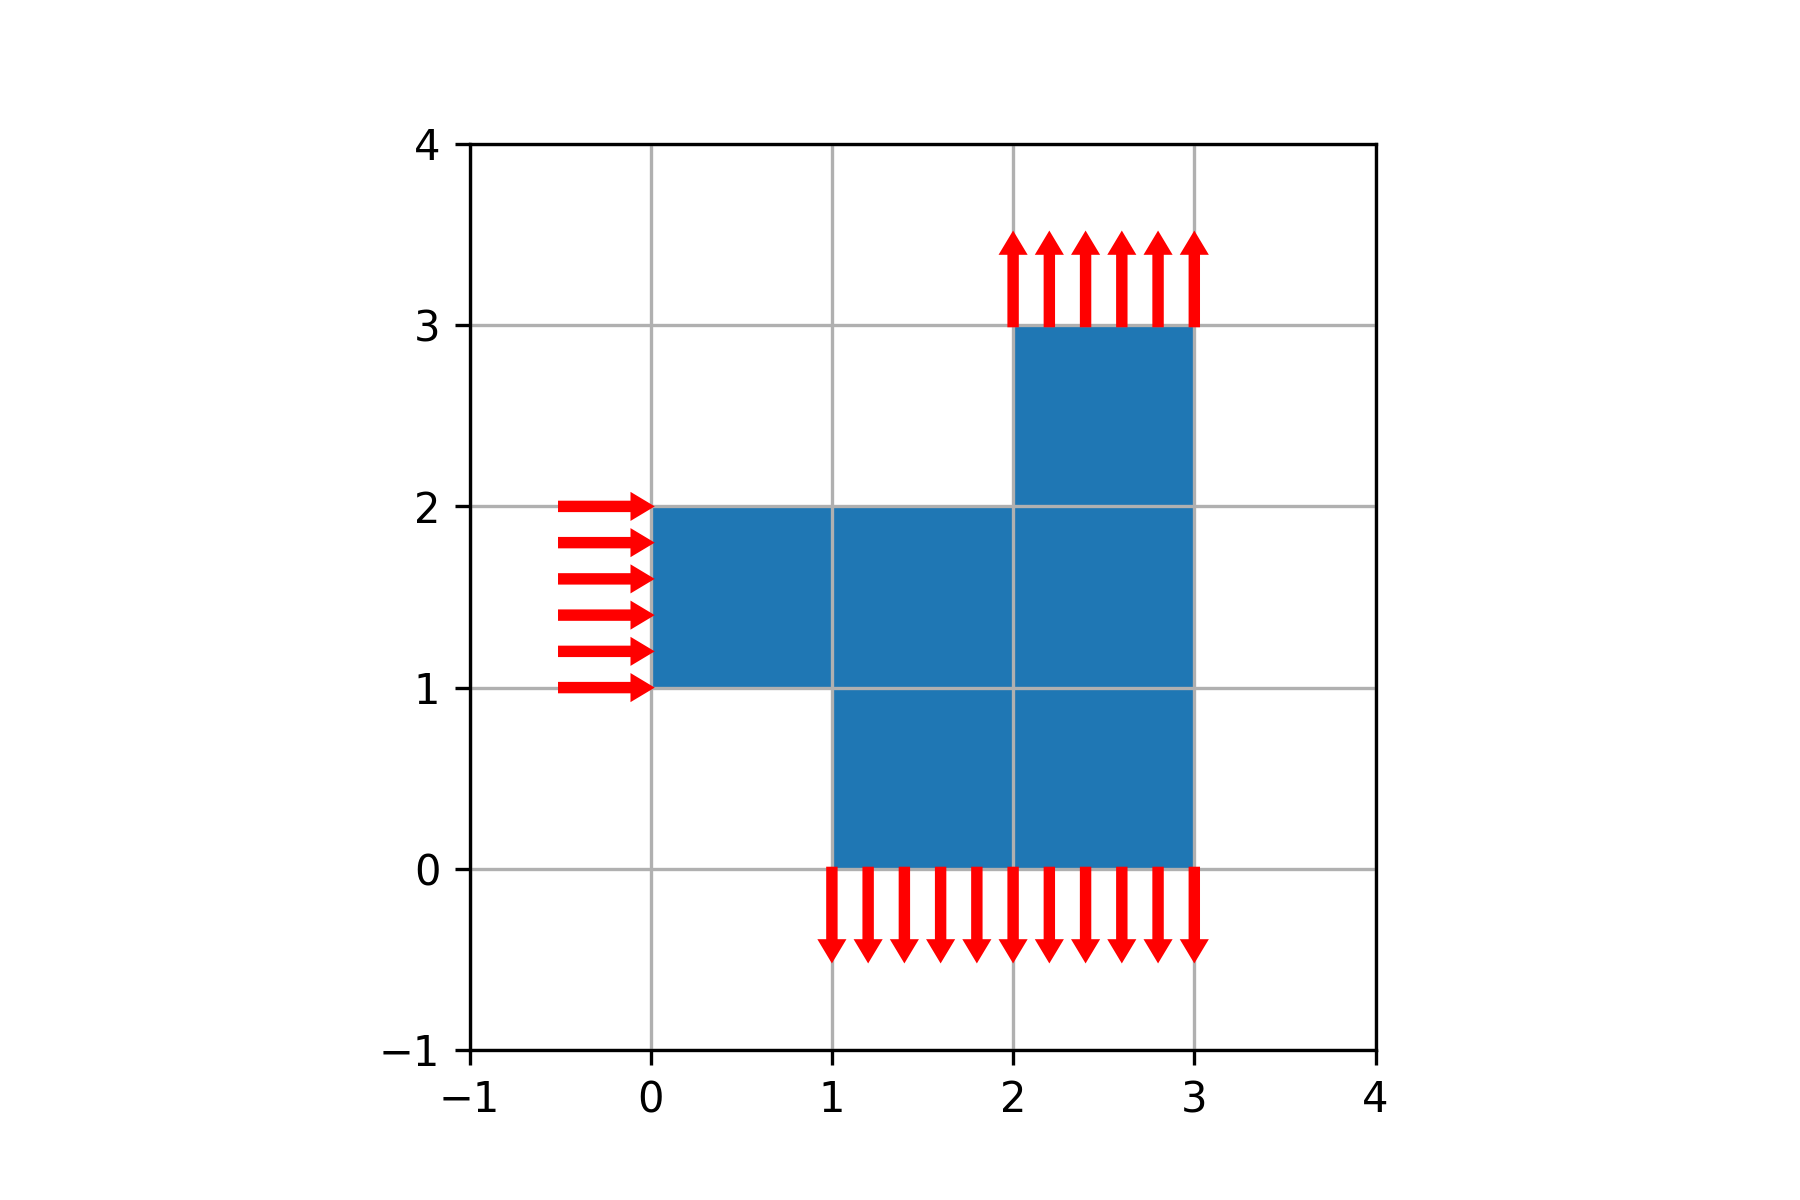
\includegraphics[]{pics/area_pic.png}
\end{figure}

Во всех заданиях в качестве области $\Omega$ будет использоваться область описанная в данном разделе.
